\documentclass[11pt]{article}

\usepackage[utf8]{inputenc}
\usepackage[T1]{fontenc}
\usepackage{lmodern}
\usepackage[margin=1in]{geometry}
\usepackage{amsmath,amssymb,amsthm,mathtools}
\usepackage{booktabs}
\usepackage{graphicx}
\usepackage{subcaption}
\usepackage{hyperref}
\usepackage{xcolor}

\hypersetup{
    colorlinks=true,
    linkcolor=blue!50!black,
    citecolor=blue!50!black,
    urlcolor=blue!50!black
}

\graphicspath{
    {../../outputs/}
    {../../doc/old/figures/cld/}
    {../figures/}
}

\newtheorem{definition}{Definition}
\newtheorem{theorem}{Theorem}
\newtheorem{proposition}{Proposition}
\newtheorem{corollary}{Corollary}
\newtheorem{remark}{Remark}
\newtheorem{assumption}{Assumption}
\newtheorem{example}{Example}
\newtheorem{lemma}{Lemma}

\newcommand{\E}{\mathbb{E}}
\newcommand{\Prob}{\mathbb{P}}
\newcommand{\R}{\mathbb{R}}
\newcommand{\X}{\mathcal{X}}
\newcommand{\Y}{\mathcal{Y}}
\newcommand{\A}{\mathcal{A}}
\newcommand{\metric}{d_{\Y}}
\newcommand{\fstar}{f^\ast}
\newcommand{\concat}{\oplus}
\DeclareMathOperator*{\argmin}{arg\,min}

\title{C-TreePO: Compression Tree Preference Optimization}
\author{Mitchell Linegar et al.}
\date{February 2026}

\begin{document}
\maketitle

\begin{abstract}
Preference optimization on long documents is constrained by context limits and oracle cost.
This draft introduces \emph{Compression Tree Preference Optimization} (C-TreePO), where one \emph{Compression Tree} (C-Tree) is the fundamental unit of representation, auditing, and optimization.
The current version centers the story on a controlled Markov changepoint benchmark trained with Fourier neural operators (FNOs), because it makes the representation problem completely explicit.
Each 128-token document is generated by a hidden stay/switch process with regime-specific vocabularies, and the root target is the number of regime transitions.
A flat FNO that reads the whole document learns this task well.
The empirical point of the draft is that a tree model with the same one-leaf FNO core can match or beat that flat baseline while observing root labels on only a subset of training documents and reallocating the missing supervision mass to count labels on some leaves.
This gives a concrete instance of the paper's broader claim: if the tree objective preserves the right local state and aggregates it correctly, partial local supervision can substitute for more expensive full-document supervision.
The remainder of the paper states the local laws, connects them to DPO/GRPO-style objectives, and gives design-based audit and certificate results.
\end{abstract}

\section{Introduction}\label{sec:introduction}

Long-document preference optimization presents a practical contradiction. The quality signal we care about is global and often interaction-heavy, while oracle access is local, expensive, and context-limited. Full-document comparisons are accurate but costly; truncation is cheaper but can distort the utility that defines the learning problem. The central question is therefore structural: \emph{can we decompose optimization so that local checks still control global preference behavior?}

C-TreePO answers this question by replacing ``one long context'' with a recursively constructed \emph{Compression Tree}. An individual tree instance is a \textbf{C-Tree}, and the method family is \textbf{C-TreePO} (Compression Tree Preference Optimization). Each node stores a bounded summary state, optimization and auditing are performed over these states, and guarantees are written as explicit statements about oracle discrepancy between original documents and tree outputs. At system scale, multiple C-Trees form the \textbf{Semantic Forests} layer, which is the natural focus of a separate systems paper.

This draft now makes the representation question concrete through one controlled benchmark rather than a menu of small toy checks. We use a flat Fourier neural operator (FNO) as the baseline long-context learner. Most readers will not already have FNOs in mind, so the operational description is simple: an FNO is a neural operator that reads an entire discretized sequence, mixes information globally in Fourier space, and maps that whole object to a prediction. In our setting it is the cleanest flat model of ``read all 128 tokens and predict the document-level target.''

Why a constructed benchmark instead of human preferences first? Because we want an exact oracle. Each document in the benchmark is generated by a hidden Markov color process with regime-specific vocabularies, and the target is the number of regime changes. From this scalar oracle one can induce pairwise or listwise preferences if desired, but the core representation problem is already present at the scalar level: can local supervision teach a tree to preserve the same root object that a strong flat operator learns from whole-document access?

The main empirical finding is simple. The flat FNO learns the task well. Yet once the tree objective is augmented with local count supervision and the predictions are aggregated hierarchically, the tree can match or outperform that same-budget flat baseline even when only a subset of training documents receive root labels and the remaining supervision mass is spent on some leaves. This is exactly the kind of phenomenon C-TreePO is meant to explain.

The reading order is therefore as follows. Section~\ref{sec:mergeable-intuition} gives a gentle description of the Markov/FNO environment and the supervision geometry. Section~\ref{sec:semantic-lift} explains what that benchmark teaches us about C-Trees more generally. The core C-TreePO method and guarantees are then stated in Sections~\ref{sec:po-mapping}--\ref{sec:estimation}.

\section{Framework and Local Laws}\label{sec:framework}

\subsection{Setup}

We now fix the main-text setup as explicitly as possible. Let $x\in\X$ be a document, let $g$ be a (possibly stochastic) compression operator, and let $\fstar:\X\to\Y$ be the oracle returning task values of interest. A C-Tree applies $g$ at leaves and then recursively on concatenated child summaries. We compare strings in oracle space with metric $\metric$.

\begin{assumption}[Fixed C-Tree Structure]\label{ass:fixed-structure}
For each document $x$, the C-Tree topology and leaf partition are treated as fixed throughout optimization and auditing in the main text.
\end{assumption}

Assumption~\ref{ass:fixed-structure} is a notational simplification, not a restriction of principle. It isolates representation quality from partition randomness so the local-to-global argument can be read directly. Appendix~\ref{app:fixed-partition} then shows the same preservation logic holds for any deterministic partition rule that maps each document to a fixed realized tree.

\begin{definition}[Oracle Equivalence]
For strings/spans $u,v$, define $u\sim v$ iff $\metric(\fstar(u),\fstar(v))=0$.
\end{definition}

\begin{assumption}[Context Compatibility]\label{ass:context-compat}
For all strings $u,v,w$, if $u\sim v$ then both $w\concat u\sim w\concat v$ and $u\concat w\sim v\concat w$.
\end{assumption}

The C-Tree audit uses three local consistency laws. They are written locally because each is checked on bounded prompts, but together they imply global control over the tree output:
\begin{align*}
\text{(C1) Sufficiency:}\quad & g(b)\sim b\quad\text{for every realized leaf }b,\\
\text{(C2) Idempotence:}\quad & g(s)\sim s\quad\text{for every }s\in\operatorname{range}(g),\\
\text{(C3) Merge Consistency:}\quad &
u\concat v\sim g(u\concat v)\sim g\big(g(u)\concat g(v)\big)\quad\text{for all }u,v.
\end{align*}

The role of each law is operational. C1 asserts that a leaf summary preserves oracle-relevant content. C2 prevents drift when already-compressed states are reprocessed. C3 is the compositional law that allows local guarantees to propagate upward through internal merges.

\begin{figure}[t]
    \centering
    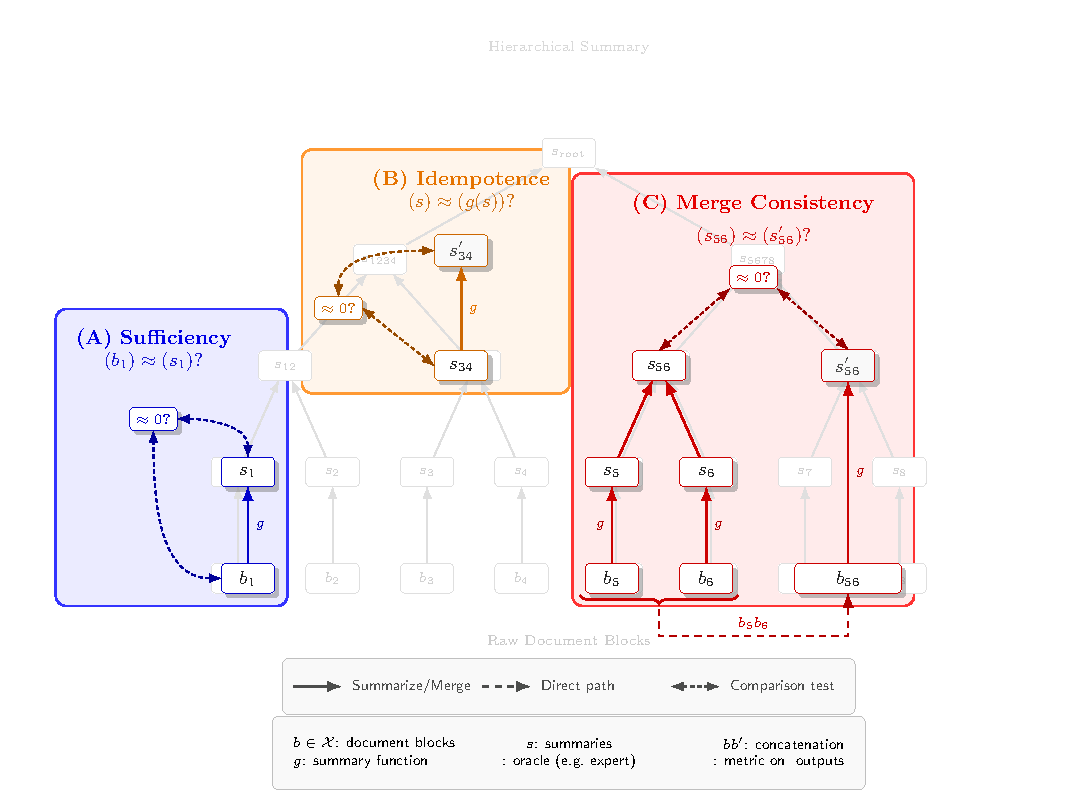
\includegraphics[width=0.95\linewidth]{05_full.pdf}
    \caption{Spotlight view of the three local laws on a realized tree.
    Gray nodes are context; colored panels are the auditable local prompts.
    This is the operational object for both certification and optimization.}
    \label{fig:local-laws-full}
\end{figure}

\begin{figure}[t]
    \centering
    \begin{subfigure}[b]{0.32\linewidth}
        \centering
        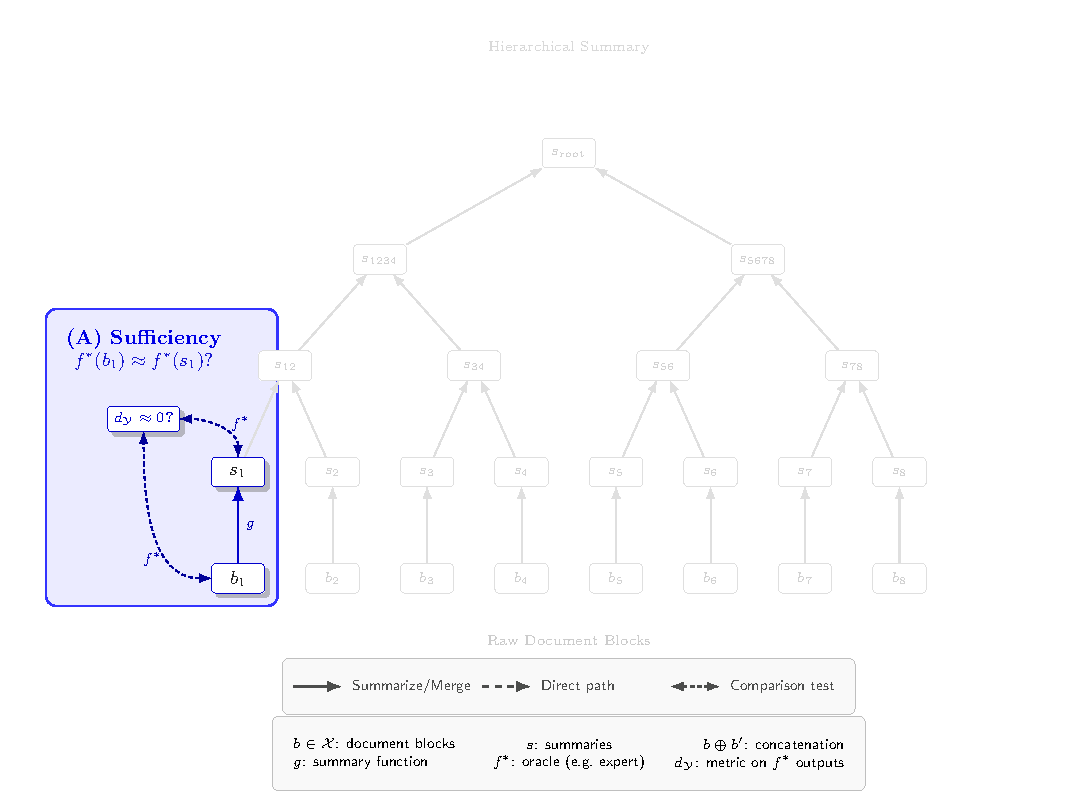
\includegraphics[width=\linewidth]{02_sufficiency.pdf}
        \caption{C1}
    \end{subfigure}
    \hfill
    \begin{subfigure}[b]{0.32\linewidth}
        \centering
        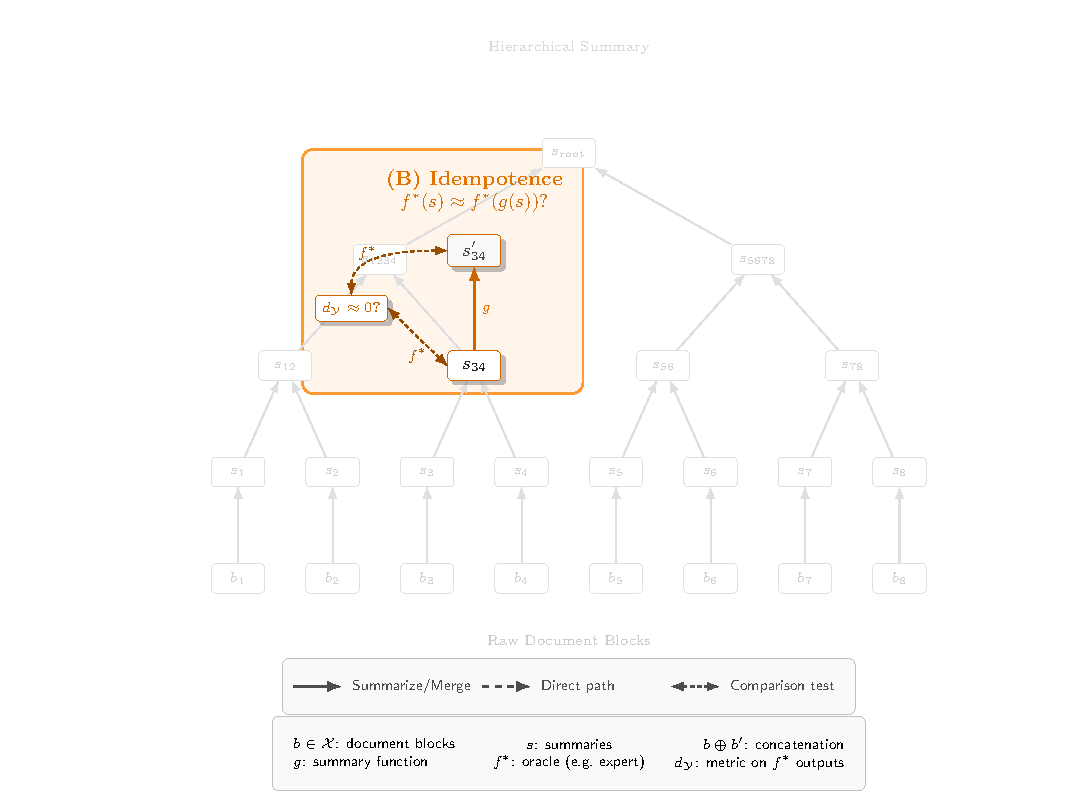
\includegraphics[width=\linewidth]{03_idempotence.pdf}
        \caption{C2}
    \end{subfigure}
    \hfill
    \begin{subfigure}[b]{0.32\linewidth}
        \centering
        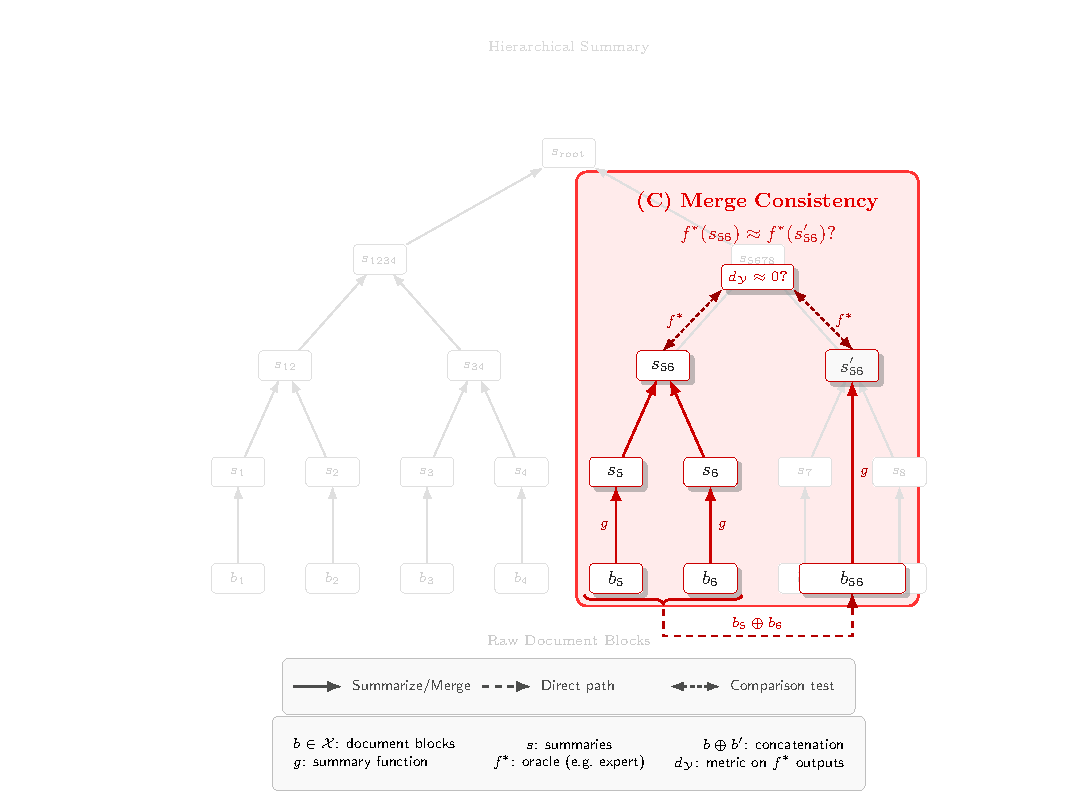
\includegraphics[width=\linewidth]{04_merge.pdf}
        \caption{C3}
    \end{subfigure}
    \caption{Law-specific panels reused from the slides.
    Each panel corresponds to a bounded context that can be sampled and scored.}
    \label{fig:local-laws-panels}
\end{figure}

\subsection{Proof Strategy}

The paper's proofs are intentionally constructive. Each global claim is decomposed into local invariance steps involving tree structure, oracle measurability, and design-based estimation, then recomposed by induction or triangle inequality. To make this auditable, Appendix~\ref{app:proof-map} provides a map from each result to its full proof location, and each appendix proof cites the corresponding Lean theorem anchors.

\section{A Gentle Markov/FNO Learning Environment}\label{sec:mergeable-intuition}

\subsection{Why start with an FNO?}

The current paper needs one benchmark that is both strong enough to be interesting and simple enough to explain from first principles. A Fourier neural operator provides exactly that benchmark. In our setting, the FNO is a flat long-context learner: it reads the entire 128-token document at once and predicts the document-level target directly. The tree model is then compared to a serious non-tree baseline rather than to a deliberately weak bag-of-leaves surrogate.

This benchmark is also a clean learning environment for oracle-indexed preferences. If we want a pairwise task, we can define $x^+ \succ x^-$ whenever the oracle score on $x^+$ exceeds the oracle score on $x^-$. If we want a scalar task, we can train directly on the oracle score itself. Either way, the representation question is the same: what local state has to survive in the tree so that the root prediction preserves the oracle object?

\subsection{The constructed color-transition task}

Each document has exactly $T=128$ token positions. There is an unobserved regime sequence
\[
z_{1:T}\in\{1,\dots,R\}^{128},
\]
which one can think of as hidden colors. In the simple benchmark, $R=4$. Each color owns its own disjoint palette of four synonymous surface tokens, so the total observed vocabulary size is $16$. The learner sees only the surface tokens, not the hidden color ids.

The generator is a symmetric stay/switch hazard process. We sample $z_1$ uniformly from the $R$ regimes, and then for each $t\ge2$:
\[
z_t=
\begin{cases}
z_{t-1}, & \text{with probability }1-p,\\
\text{Unif}\big(\{1,\dots,R\}\setminus\{z_{t-1}\}\big), & \text{with probability }p.
\end{cases}
\]
Conditional on $z_t=r$, the observed token is emitted from a regime-specific categorical distribution $\phi_r$ supported only on that regime's four-token palette.

The oracle target is the total number of regime changes:
\[
\fstar(x)=y(x):=\sum_{t=1}^{127}\mathbf{1}\{z_t\neq z_{t+1}\}.
\]
Equivalently, the model is asked to count how many times the hidden color changes across the document. In the recoverable benchmark we set $p=5/127$, so the expected number of changepoints is about $5$. In the harder structural benchmark we raise both the state complexity and the boundary density to $R=12$ and $p=10/127$, yielding about $10$ expected changepoints and a vocabulary of size $48$.

\begin{figure}[t]
    \centering
    \includegraphics[width=\linewidth]{markov_changepoint_dgp_slide.pdf}
    \caption{Schematic view of one toy Markov document. The figure is illustrative; the actual simple benchmark uses 128 tokens, four hidden regimes, and four synonymous surface tokens per regime. The root oracle is the number of latent regime changes.}
    \label{fig:markov-dgp}
\end{figure}

\subsection{What has to be aggregated?}

This benchmark is useful because the exact tree state is easy to write down. For any contiguous span $u$, let
\[
S(u)=\big(c(u),a(u),b(u)\big),
\]
where $c(u)$ is the number of internal changepoints in the span, $a(u)$ is the first regime in the span, and $b(u)$ is the last regime in the span. If $u_L$ and $u_R$ are adjacent child spans, then the parent state is
\[
S(u_L\concat u_R)=\Big(c(u_L)+c(u_R)+\mathbf{1}\{b(u_L)\neq a(u_R)\},\ a(u_L),\ b(u_R)\Big).
\]

This is the whole aggregation story in one line. The root count is \emph{not} additively separable in leaf-local counts alone, because there is a boundary join term $\mathbf{1}\{b(u_L)\neq a(u_R)\}$ that depends on both children. A tree therefore needs more than ``how many flips were inside this leaf?'' It also needs enough boundary information to determine whether two neighboring leaves create one more flip when they are merged.

\subsection{From the flat FNO to the tree}

The flat baseline is the direct map
\[
h_{\mathrm{flat}}:x_{1:128}\mapsto \widehat{y},
\]
implemented by a one-dimensional FNO over the full document. The tree model uses the same FNO-style encoder at the leaves, but now the encoder is applied to shorter spans and its outputs are merged upward. When the leaf size is 128, the tree has only one leaf and no merge path at all; this is the \emph{one-leaf parity canary}. If the leaf-128 tree does not agree with the flat FNO, the comparison is not fair. When the leaf size drops to 64, 32, 16, or 8, the merge path becomes active and the representation problem appears.

\begin{figure}[t]
    \centering
    \includegraphics[width=\linewidth]{markov_neural_operator_slide.pdf}
    \caption{The tree/FNO comparison in operational terms. With one leaf, the tree collapses to the flat FNO core. With multiple leaves, the model must learn leaf-local state and a merge rule that preserves the root count.}
    \label{fig:markov-operator}
\end{figure}

The benchmark lets us separate two kinds of supervision. Root supervision tells the model the final document-level count. Local supervision tells the model something about what each leaf should emit before the tree is merged. In the current experiments, a full-document root label contributes mass $1$, while a label on a leaf of length $\ell$ contributes mass $\ell/128$. If the training set contains $N=10{,}240$ documents and only a fraction $\rho$ receive root labels, then the root-only budget is $\rho N$. In the equal-total-mass comparison we reallocate the missing $(1-\rho)N$ units of supervision mass to leaf labels, which means
\[
\#\text{added leaf labels}=(1-\rho)N\cdot \frac{128}{\ell}.
\]
For $\ell=8$, one missing root label can therefore be replaced by sixteen count-only leaf labels. This is the supervision geometry behind the result tables below.

\section{What the Markov Benchmark Teaches About C-Trees}\label{sec:semantic-lift}

The Markov example is not the application of C-TreePO; it is the cleanest controlled environment we have for seeing what a compression tree has to preserve. The lesson is structural. A useful tree state is not whatever happens to predict well locally. It is the state that makes the root object compositional under merges. In the changepoint benchmark, that state is ``internal count plus enough boundary information to know whether a new count is created at the join.'' In a semantic task, the analogue is not literally first and last regimes, but some task-specific boundary-sensitive information that determines how two spans interact when they are combined.

This gives a more concrete version of non-separability than a generic toy threshold. If we keep only leaf-local counts and discard the boundary variables, then the root objective is no longer computable from leaf outputs alone. The join term is precisely the sort of interaction-bearing information that C3 is supposed to protect.

\begin{definition}[Additively Separable and Not Additively Separable Tree Utilities]\label{def:nonseparable}
A tree-level utility $U$ is additively separable if there exist leaf-local functions $\{h_u\}$ such that
\[
U(T)=\sum_{u\in\mathrm{Leaves}(T)} h_u(s_u)
\]
for all realized trees in the support. A utility is not additively separable when no such representation exists and interaction terms are required.
\end{definition}

\begin{example}[Markov changepoint utility is not separable in leaf counts alone]\label{ex:threshold-nonseparable}
Let two child summaries carry exact states
\[
s_L=(c_L,a_L,b_L),\qquad s_R=(c_R,a_R,b_R),
\]
and define the parent count utility by
\[
U(s_L,s_R)=c_L+c_R+\mathbf{1}\{b_L\neq a_R\}.
\]
If we retain only $(c_L,c_R)$, the join term is missing and the root count is unidentified. Once we retain the boundary variables $(a_L,b_L,a_R,b_R)$ as well, the parent utility becomes exactly compositional. The semantic analogue is a claim-evidence or premise-conclusion pair where neither span alone determines the downstream judgment, but the boundary relation between the two spans does.
\end{example}

For this reason C-TreePO is not a bag-of-node surrogate. The tree utility must allow interaction terms, and the role of the local laws is to preserve exactly the interaction-bearing information needed by the oracle objective:
\[
U(T)=\sum_{u\in T}\phi_u + \sum_{(u,v)\in\mathcal{E}(T)}\psi_{uv} + \sum_{p\in\mathcal{P}(T)}\chi_p,
\]
where $\psi_{uv}$ and $\chi_p$ capture sibling and path interactions.

The Markov benchmark also clarifies what the partial-leaf-label result does and does not mean. The tree does not win because we secretly give it a second copy of the root label. In fact, duplicating the document count onto a single leaf is a poor baseline. The tree wins when local supervision teaches a useful decomposition of the root object and the merge rule can aggregate those local predictions coherently. That is the broad C-TreePO point in miniature.

\section{C-TreePO as Preference Optimization}\label{sec:po-mapping}

\subsection{Data-generating object}

For document $x$, Assumption~\ref{ass:fixed-structure} gives a fixed realized tree structure, and policy $\pi_\theta$ induces randomness only through node-level generation, compression, and scoring decisions on that structure. We write the resulting random C-Tree as $T\sim\pi_\theta(\cdot\mid x)$:
\[
T = \mathrm{BuildTree}(x,\mathcal{T}(x);\theta,\xi),
\]
where $\xi$ denotes internal stochasticity. Preference supervision is collected over paired trees $(T^+,T^-)$.

The same formal mapping extends to any deterministic partition rule $\Pi$ with $x\mapsto\mathcal{T}_\Pi(x)$, because conditioning on $\mathcal{T}_\Pi(x)$ returns the identical fixed-structure argument. Appendix~\ref{app:fixed-partition} gives the explicit statement and proof.

\subsection{Objective layer}

For pairwise optimization (DPO style), the tree-level objective is:
\[
\mathcal{L}_{\mathrm{DPO}}(\theta)
= -\E\!\left[\log\sigma\!\left(
\beta\log\frac{\pi_\theta(T^+\mid x)}{\pi_{\mathrm{ref}}(T^+\mid x)}
-\beta\log\frac{\pi_\theta(T^-\mid x)}{\pi_{\mathrm{ref}}(T^-\mid x)}
\right)\right].
\]
Listwise and RL-style objectives use tree groups and tree-indexed rank/reward definitions analogously.

\subsection{Core guarantees}

\begin{theorem}[Preservation Under Local Laws]\label{thm:preservation}
Assume C1--C3 hold on realized C-Tree leaves and internal edges.
Then the expected oracle distortion between the C-Tree output and the original document is zero:
\[
\E\left[\metric\big(\fstar(Z^{(R)}(x)),\fstar(x)\big)\right]=0\quad\text{for }R\ge1.
\]
\end{theorem}

The proof is inductive over tree structure and rounds. C1 handles leaves, C3 transports equivalence across merges, and C2 controls re-summarization rounds. The corresponding Lean theorem is \texttt{multi\_round\_proper}.

\begin{theorem}[Preference-Objective Equivalence]\label{thm:equiv}
Under oracle-measurability/indexing conditions for policies, generators, and rewards/rankers,
training objectives on C-Tree summaries equal corresponding objectives on originals.
For nonzero distortion $\Delta_R$, objective differences satisfy method-specific Lipschitz bounds:
\[
\left|\E[\mathcal{L}(X)]-\E[\mathcal{L}(Z)]\right| \le L\,\Delta_R.
\]
\end{theorem}

Lean anchors for Theorem~\ref{thm:equiv} are \texttt{dpo\_equivalence}, \texttt{grpo\_equivalence}, \texttt{grpo\_rl\_equivalence}, and \texttt{unified\_preference\_gap\_bounded}.

\begin{theorem}[End-to-End C-TreePO Certificate]\label{thm:e2e}
With logged propensities and design-based sampling,
Horvitz--Thompson style estimators of C-Tree objective terms are unbiased (or controlled in clipped/noisy variants),
and method-level DPO/GRPO gap certificates follow by composition.
\end{theorem}

\subsection{Map of Full Proofs}

Table~\ref{tab:proof-map-main} shows where each complete proof appears in the appendix.
The detailed theorem-to-Lean crosswalk is moved to Appendix~\ref{app:lean-crosswalk}.
A supporting extension theorem covering arbitrary deterministic fixed partition rules appears in Appendix~\ref{app:fixed-partition}.

\begin{table}[t]
\centering
\small
\begin{tabular}{p{0.42\linewidth}p{0.45\linewidth}}
\toprule
Result in Main Text & Full proof location \\
\midrule
Theorem~\ref{thm:preservation} (local laws $\Rightarrow$ preservation) & Appendix~\ref{app:proof-preservation} \\
Theorem~\ref{thm:equiv} (preference-objective equivalence and gap bound) & Appendix~\ref{app:proof-equivalence} \\
Theorem~\ref{thm:e2e} (end-to-end certificate) & Appendix~\ref{app:proof-e2e} \\
\bottomrule
\end{tabular}
\caption{Map of where each full proof is written out in detail.}
\label{tab:proof-map-main}
\end{table}

C-TreePO is best described as a compression-tree data and estimation framework that enables standard preference optimizers with explicit distortion and estimation certificates.

\section{Markov/FNO Results}\label{sec:empirics}

All panels in this section fix the training set size at $10{,}240$ documents and sweep two design choices: the fraction of documents that receive root labels ($R100$ down to $R10$) and the tree leaf size (128, 64, 32, 16, or 8 tokens, corresponding to 1, 2, 4, 8, or 16 leaves). The amber horizontal baseline in each panel is the matched flat FNO trained on the same number of root-labeled documents. The leaf-128 tree point is the one-leaf parity canary discussed above: if it does not line up with the flat FNO, the tree/FNO comparison is not trustworthy.

\subsection{Recoverable four-regime benchmark}

Figure~\ref{fig:recoverable-markov} shows the simple case: four hidden regimes, a vocabulary of sixteen observed tokens (four synonyms per regime), and switch probability $p=5/127$. The qualitative pattern is clean.

First, the leaf-128 parity canary agrees with the flat FNO throughout the sweep, which is the sanity check we need. Second, once real tree structure is allowed, the best root-only tree beats the same-budget flat FNO at every root-label budget. Third, reallocating the missing supervision mass to count labels on some leaves is not necessary for the tree to beat FNO, but it does help in the low-budget regime. The most striking example is $R10$: the best root-only tree reaches MAE $0.469$, the flat FNO is at $1.227$, and the equal-total-mass leaf-label tree improves further to $0.428$.

\begin{figure}[t]
    \centering
    \begin{subfigure}[b]{0.49\linewidth}
        \centering
        \includegraphics[width=\linewidth]{markov_v5_simple_current_plots_20260415_205235/figures/recoverable_root_only_leaf_size_fixed_train10240.png}
        \caption{Root-only supervision.}
    \end{subfigure}
    \hfill
    \begin{subfigure}[b]{0.49\linewidth}
        \centering
        \includegraphics[width=\linewidth]{markov_v5_simple_current_plots_20260415_205235/figures/recoverable_root_only_leaf_size_fixed_with_leaf_mass_equivalent_train10240.png}
        \caption{Root-only plus equal-total-mass leaf labels.}
    \end{subfigure}
    \caption{Recoverable Markov benchmark with $10{,}240$ training documents. The flat FNO is strong, but once the tree is allowed to use real multi-leaf structure it stays substantially below the matched FNO error across the whole root-budget sweep. The blue series shows what happens when missing root supervision mass is reallocated to count labels on some leaves.}
    \label{fig:recoverable-markov}
\end{figure}

\begin{table}[t]
    \centering
    \small
    \resizebox{\linewidth}{!}{%
    \begin{tabular}{lccccc}
        \toprule
        Root budget & Best root leaf & Best root MAE & Flat FNO MAE & Best leaf-mass leaf & Best leaf-mass MAE \\
        \midrule
        R100 & 8 & 0.198 & 0.496 & 8 & 0.198 \\
        R90 & 8 & 0.198 & 0.523 & 8 & 0.196 \\
        R80 & 8 & 0.199 & 0.508 & 8 & 0.221 \\
        R70 & 8 & 0.205 & 0.672 & 8 & 0.209 \\
        R60 & 8 & 0.219 & 0.730 & 8 & 0.228 \\
        R50 & 8 & 0.251 & 0.707 & 8 & 0.252 \\
        R40 & 8 & 0.277 & 0.867 & 64 & 0.312 \\
        R30 & 64 & 0.330 & 1.000 & 64 & 0.314 \\
        R20 & 64 & 0.342 & 1.098 & 64 & 0.354 \\
        R10 & 64 & 0.469 & 1.227 & 64 & 0.428 \\
        \bottomrule
    \end{tabular}
    }
    \caption{Recoverable benchmark summary. ``Best root'' is the best root-only tree at that budget; ``best leaf-mass'' is the best tree after reallocating the missing root supervision mass to count-only leaf labels.}
    \label{tab:recoverable-markov}
\end{table}

Two diagnostics matter for interpretation. The first is that the smallest leaves dominate the moderate- and high-budget region: leaf size 8 is best from $R100$ through $R40$. Only when root labels become very scarce does the optimum move back to a coarser geometry (leaf 64), which is the expected bias-variance tradeoff. The second is that naive label duplication is \emph{not} the explanation. In the one-leaf case, simply attaching the document count again as a local count-only target is often very poor (for example, MAE $1.797$ at $R50$, $R30$, and $R10$), so the gain is coming from actual tree structure and useful local decomposition, not from copying the root label into a second loss term.

\subsection{Harder structural benchmark}

Figure~\ref{fig:structural-markov} keeps the same document length and task but makes the latent process materially harder: twelve hidden regimes, vocabulary size $48$, and switch probability $p=10/127$. The main ordering survives. The best root-only tree still beats the flat FNO at every budget, and partial leaf labels still help in several mid-budget panels. What changes is the size and stability of the gain. Absolute error is higher, the optimal leaf size moves around more, and the equal-total-mass leaf-label improvement is smaller and less uniform.

\begin{figure}[t]
    \centering
    \begin{subfigure}[b]{0.49\linewidth}
        \centering
        \includegraphics[width=\linewidth]{markov_v5_simple_current_plots_20260415_205235/figures/structural_root_only_leaf_size_fixed_train10240.png}
        \caption{Root-only supervision.}
    \end{subfigure}
    \hfill
    \begin{subfigure}[b]{0.49\linewidth}
        \centering
        \includegraphics[width=\linewidth]{markov_v5_simple_current_plots_20260415_205235/figures/structural_root_only_leaf_size_fixed_with_leaf_mass_equivalent_train10240.png}
        \caption{Root-only plus equal-total-mass leaf labels.}
    \end{subfigure}
    \caption{Harder structural benchmark with twelve hidden regimes and higher boundary density. The tree still dominates the matched flat FNO, but the margin is smaller and the best leaf geometry is less stable.}
    \label{fig:structural-markov}
\end{figure}

\begin{table}[t]
    \centering
    \small
    \resizebox{\linewidth}{!}{%
    \begin{tabular}{lccccc}
        \toprule
        Root budget & Best root leaf & Best root MAE & Flat FNO MAE & Best leaf-mass leaf & Best leaf-mass MAE \\
        \midrule
        R100 & 16 & 0.829 & 1.254 & 16 & 0.829 \\
        R90 & 32 & 0.850 & 1.410 & 16 & 0.858 \\
        R80 & 16 & 0.874 & 1.332 & 8 & 0.881 \\
        R70 & 8 & 0.873 & 1.574 & 16 & 0.869 \\
        R60 & 8 & 0.940 & 1.652 & 8 & 0.933 \\
        R50 & 16 & 0.942 & 1.762 & 8 & 0.929 \\
        R40 & 8 & 0.936 & 2.027 & 8 & 0.920 \\
        R30 & 8 & 0.983 & 2.227 & 8 & 0.975 \\
        R20 & 8 & 1.076 & 2.418 & 8 & 1.097 \\
        R10 & 64 & 1.212 & 2.426 & 64 & 1.232 \\
        \bottomrule
    \end{tabular}
    }
    \caption{Hard structural benchmark summary. The tree keeps a large edge over the flat FNO, but the residual difficulty gap is real and the partial-leaf-count advantage is less uniform than in the recoverable four-regime case.}
    \label{tab:structural-markov}
\end{table}

This harder case is important because it prevents the story from being oversold. The simple benchmark is not a degenerate one-leaf parity artifact: the leaf-128 canary behaves correctly, and the gains appear only once the tree is allowed to use genuine multi-leaf structure. But the hard benchmark shows that the method still has headroom. The tree wins, partial leaf counts sometimes help further, and the remaining gap now looks like a real representational and optimization problem rather than a bookkeeping issue.

\section{Estimation, Auditing, and Honesty}\label{sec:estimation}

C-TreePO relies on sampled oracle queries.
For queried unit $i$ with inclusion indicator $Z_i$, propensity $\pi_i$, and contribution $R_i$, the HT estimator is:
\[
\hat{J}_{\mathrm{HT}} = \frac{1}{n}\sum_i \frac{Z_i}{\pi_i}R_i.
\]

Adaptive chunking and learned judges introduce interference paths.
To keep evaluation valid, reporting must be honest with respect to adaptation roles (chunker, summarizer, oracle): adaptation on train-role partitions, evaluation on held-out role intersections.
The same discipline applies to simulation sweeps with tunable local-law weights: hyperparameter selection belongs on a validation split, and the paper's quantitative claims should be reported on a disjoint test split. Any plots that optimize on the same held-out slice they report are exploratory diagnostics rather than confirmatory evidence.

A practical bound stack decomposes target error into calibration, estimation, and clipping envelopes.
For true gap $G^\ast$, judge-view $G^J$, sampled estimate $G^E$, and clipped estimate $G^C$:
\[
|G^\ast-G^C| \le |G^\ast-G^J| + |G^J-G^E| + |G^E-G^C|.
\]
Event-based concentration and union composition then yield one-shot high-probability certificates.

\section{Scope and Relation to Semantic Forests}\label{sec:scope}

C-TreePO is intended for long-context settings in which full-document oracle usage is too expensive, local bounded checks are feasible, and utility-relevant information can be propagated through compression states.

Likely failure modes include irreducibly nonlocal tasks, severe support collapse, and unstable calibration transfer.

This paper should own the method and certificate core (local laws, objective mapping, estimation guarantees).
The Semantic Forests paper should own system-scale orchestration, deployment engineering, and broad cross-domain throughput/robustness analysis.

\section{Conclusion}\label{sec:conclusion}

C-TreePO provides a concrete local-to-global route for long-document preference optimization.
The current draft is organized around one controlled story: a flat FNO learns a Markov changepoint task well, and a tree with the same one-leaf operator can recover or improve that performance by redistributing part of the supervision budget from missing root labels to local leaf labels.
That benchmark makes the paper's main point easier to see. The issue is not generic compression; it is preservation of the local state needed to aggregate into the same root object.
The formal contribution of C-TreePO is then to state that requirement as local laws, connect those laws to preference-objective equivalence, and turn sampled audits into explicit end-to-end certificates rather than implicit trust in truncation.

\appendix

\section{Proof Map and Lean Crosswalk}\label{app:proof-map}

\subsection{Proof Map}

\begin{table}[h]
\centering
\small
\begin{tabular}{p{0.34\linewidth}p{0.24\linewidth}p{0.36\linewidth}}
\toprule
Result & Appendix proof section & Lean reference section \\
\midrule
Theorem~\ref{thm:fixed-partition} & Appendix~\ref{app:fixed-partition} & Appendix~\ref{app:lean-crosswalk} \\
Theorem~\ref{thm:preservation} & Appendix~\ref{app:proof-preservation} & Appendix~\ref{app:lean-crosswalk} \\
Theorem~\ref{thm:equiv} & Appendix~\ref{app:proof-equivalence} & Appendix~\ref{app:lean-crosswalk} \\
Theorem~\ref{thm:e2e} & Appendix~\ref{app:proof-e2e} & Appendix~\ref{app:lean-crosswalk} \\
\bottomrule
\end{tabular}
\caption{Navigation map for all full proofs in this draft.}
\end{table}

\subsection{Lean Crosswalk}\label{app:lean-crosswalk}

\begin{table}[h]
\centering
\small
\begin{tabular}{p{0.34\linewidth}p{0.30\linewidth}p{0.30\linewidth}}
\toprule
Paper result & Lean theorem name(s) & Lean file \\
\midrule
Theorem~\ref{thm:fixed-partition} &
\texttt{multi\_round\_proper} (instantiated for arbitrary fixed tree) &
\texttt{lean3/FormalProofs/OPT/ExpectationTheory.lean} \\

Theorem~\ref{thm:preservation} &
\texttt{multi\_round\_proper} &
\texttt{lean3/FormalProofs/OPT/ExpectationTheory.lean} \\

Theorem~\ref{thm:equiv} (exact case) &
\texttt{dpo\_equivalence}, \texttt{grpo\_equivalence}, \texttt{grpo\_rl\_equivalence} &
\texttt{lean3/FormalProofs/OPT/PreferenceLearning.lean} \\

Theorem~\ref{thm:equiv} (gap bound) &
\texttt{unified\_preference\_gap\_bounded} &
\texttt{lean3/FormalProofs/OPT/PreferenceBounds.lean} \\

Theorem~\ref{thm:e2e} (objective unbiasedness) &
\texttt{treepo\_objective\_unbiased}, \texttt{treepo\_distortion\_unbiased} &
\texttt{lean3/FormalProofs/DSL/TreePOEndToEnd.lean} \\

Theorem~\ref{thm:e2e} (method certificates) &
\texttt{dpo\_treepo\_end\_to\_end\_certificate}, \texttt{grpo\_pl\_treepo\_end\_to\_end\_certificate}, \texttt{grpo\_rl\_treepo\_end\_to\_end\_certificate} &
\texttt{lean3/FormalProofs/DSL/TreePOEndToEnd.lean} \\

Sketch-transport component used in Theorem~\ref{thm:e2e} discussion &
\texttt{dpo\_tree\_gap\_bounded\_by\_sketch\_upper}, \texttt{grpo\_pl\_tree\_gap\_bounded\_by\_sketch\_upper}, \texttt{grpo\_rl\_tree\_gap\_bounded\_by\_sketch\_upper} &
\texttt{lean3/FormalProofs/DSL/MergeableCertificates.lean} \\
\bottomrule
\end{tabular}
\caption{Theorem-to-Lean crosswalk (moved to appendix).}
\end{table}

\section{Fixed-Partition Extension}\label{app:fixed-partition}

\begin{theorem}[Extension to Any Deterministic Fixed Partition]\label{thm:fixed-partition}
Let $\Pi$ be any deterministic rule that maps each document $x$ to a finite ordered rooted tree $\mathcal{T}_\Pi(x)$ with contiguous leaves. For each $x$, construct C-Tree summaries on $\mathcal{T}_\Pi(x)$ and assume C1--C3 hold almost surely on all realized leaf and merge calls. Then for every round $R\ge 1$,
\[
\E\!\left[\metric\!\big(\fstar(Z_\Pi^{(R)}(x)),\fstar(x)\big)\,\middle|\,x\right]=0.
\]
Consequently, for any distribution over documents $X$,
\[
\E\!\left[\metric\!\big(\fstar(Z_\Pi^{(R)}(X)),\fstar(X)\big)\right]=0.
\]
\end{theorem}

\begin{proof}
Fix $x$ and condition on the realized tree $\mathcal{T}_\Pi(x)$. Because $\Pi$ is deterministic, the tree is fixed under this conditioning, so Theorem~\ref{thm:preservation} applies directly and yields
\[
\E\!\left[\metric\!\big(\fstar(Z_\Pi^{(R)}(x)),\fstar(x)\big)\,\middle|\,x,\mathcal{T}_\Pi(x)\right]=0.
\]
Since $\mathcal{T}_\Pi(x)$ is a measurable function of $x$, the same equality holds conditioning only on $x$. Taking expectation over $X$ and applying the tower property gives the unconditional statement.
\end{proof}

Lean correspondence for Theorem~\ref{thm:fixed-partition} follows from the same formal theorem used in Theorem~\ref{thm:preservation}, namely \texttt{multi\_round\_proper} in \texttt{lean3/FormalProofs/OPT/ExpectationTheory.lean}, instantiated at an arbitrary fixed tree.

\section{Full Proof of Theorem~\ref{thm:preservation}}\label{app:proof-preservation}

\begin{proof}
Fix a realized full binary C-Tree $T$ over document $x$.
For each node $u$, define latent raw span $S(u)$ recursively by setting $S(u)=b$ when $u$ is a leaf containing block $b$, and setting $S(u)=S(u_L)\concat S(u_R)$ when $u$ is an internal node with children $(u_L,u_R)$.
Define stored summary $s_u$ recursively by setting $s_u=g(S(u))$ at leaves and $s_u=g(s_{u_L}\concat s_{u_R})$ at internal nodes.
Let $r$ be the root and set $Z^{(1)}(x):=s_r$.
Assume C1--C3 hold almost surely on all realized calls.

We first show $s_u\sim S(u)$ for every node $u$ by structural induction on node height. If $u$ is a leaf, C1 gives $s_u=g(S(u))\sim S(u)$. For the inductive step, assume $s_{u_L}\sim S(u_L)$ and $s_{u_R}\sim S(u_R)$.
By context compatibility,
\[
s_{u_L}\concat s_{u_R}\sim S(u_L)\concat S(u_R)=S(u).
\]
By C3 (applied to $u=s_{u_L}$ and $v=s_{u_R}$),
\[
g(s_{u_L}\concat s_{u_R})\sim s_{u_L}\concat s_{u_R}.
\]
Since $s_u=g(s_{u_L}\concat s_{u_R})$, transitivity gives $s_u\sim S(u)$.
This completes induction.

At root $r$, we have $s_r\sim S(r)=x$, hence
\[
\metric\!\big(\fstar(Z^{(1)}(x)),\fstar(x)\big)=0
\]
almost surely, so
\[
\E\!\left[\metric\!\big(\fstar(Z^{(1)}(x)),\fstar(x)\big)\right]=0.
\]

Define rounds by $Z^{(R+1)}(x):=g(Z^{(R)}(x))$ for $R\ge1$.
Because $Z^{(1)}(x)=s_r\in\operatorname{range}(g)$ and $g$ maps into its range, each $Z^{(R)}(x)$ is in $\operatorname{range}(g)$.
By C2:
\[
Z^{(R+1)}(x)\sim Z^{(R)}(x)\quad\text{for all }R\ge1.
\]
We prove $Z^{(R)}(x)\sim x$ by induction on $R$.
Base $R=1$ holds from the nodewise equivalence argument above.
If $Z^{(R)}(x)\sim x$ and $Z^{(R+1)}(x)\sim Z^{(R)}(x)$, transitivity yields $Z^{(R+1)}(x)\sim x$.
Thus $Z^{(R)}(x)\sim x$ for all $R\ge1$, so
\[
\E\!\left[\metric\!\big(\fstar(Z^{(R)}(x)),\fstar(x)\big)\right]=0.
\]
This proves Theorem~\ref{thm:preservation}.
\end{proof}

The formal theorem for this statement is
\texttt{multi\_round\_proper} in
\texttt{lean3/FormalProofs/OPT/ExpectationTheory.lean}.

\section{Full Proof of Theorem~\ref{thm:equiv}}\label{app:proof-equivalence}

\begin{proof}
Fix policy parameter $\theta$.
Let $(X,Z)$ be coupled random variables on a common probability space, with
$Z=Z^{(R)}(X)$ from the C-Tree pipeline.
Let $\mathcal{J}_\theta(x)$ denote the population integrand for the preference objective (pairwise, listwise, or RL variant after integrating over method-specific internal sampling).

Assume oracle-measurability/indexing in the sense that there exists measurable
$\phi_\theta$ on oracle space such that
\[
\mathcal{J}_\theta(x)=\phi_\theta(\fstar(x)).
\]
Under the exact-preservation condition from Theorem~\ref{thm:preservation},
$\fstar(Z)=\fstar(X)$ almost surely, hence
\[
\mathcal{J}_\theta(Z)=\phi_\theta(\fstar(Z))
=\phi_\theta(\fstar(X))
=\mathcal{J}_\theta(X)
\quad\text{a.s.}
\]
Taking expectation:
\[
\E[\mathcal{J}_\theta(Z)]=\E[\mathcal{J}_\theta(X)].
\]
Therefore the summary and original objectives are equal pointwise in $\theta$.
Consequently, their argmin sets are identical.

For the approximate case, assume an $L$-Lipschitz condition in oracle metric:
\[
|\mathcal{J}_\theta(x)-\mathcal{J}_\theta(z)|
\le L\,\metric(\fstar(x),\fstar(z)).
\]
Then
\begin{align*}
\left|\E[\mathcal{J}_\theta(X)]-\E[\mathcal{J}_\theta(Z)]\right|
&\le \E\left[\left|\mathcal{J}_\theta(X)-\mathcal{J}_\theta(Z)\right|\right] \\
&\le L\,\E\left[\metric(\fstar(X),\fstar(Z))\right] \\
&=: L\,\Delta_R.
\end{align*}
This gives the unified preference gap bound.
Applying this template to DPO, GRPO-PL, and GRPO-RL yields method-specific constants and the theorem.
\end{proof}

The Lean correspondence is as follows. Exact equivalence uses
\texttt{dpo\_equivalence}, \texttt{grpo\_equivalence},
\texttt{grpo\_rl\_equivalence} in
\texttt{lean3/FormalProofs/OPT/PreferenceLearning.lean}.
The quantitative bound uses
\texttt{unified\_preference\_gap\_bounded} in
\texttt{lean3/FormalProofs/OPT/PreferenceBounds.lean}.

\section{Full Proof of Theorem~\ref{thm:e2e}}\label{app:proof-e2e}

\begin{proof}
Let $\mathcal{U}=\bigcup_x U(x)$ be the finite population of realized tree nodes for a training/evaluation population, with $N:=|\mathcal{U}|$ and each $U(x)$ containing all realized nodes of document $x$ (including the root).
For each unit $i\in\mathcal{U}$, let $Y_i$ denote a target contribution (objective or distortion term), and let $Z_i\in\{0,1\}$ be its sampling indicator with logged propensity
$\pi_i:=\Prob(Z_i=1\mid\mathcal{F})$, where $0<\pi_i\le1$.
Condition on $\mathcal{F}$ (the sigma-field generated by population values and sampling design metadata).

Define Horvitz--Thompson estimator:
\[
\widehat{\mu}_{\mathrm{HT}}:=\frac{1}{N}\sum_{i\in\mathcal{U}}\frac{Z_i}{\pi_i}Y_i.
\]
Then
\[
\E\left[\frac{Z_i}{\pi_i}Y_i\,\middle|\,\mathcal{F}\right]
=\frac{\E[Z_i\mid\mathcal{F}]}{\pi_i}Y_i
=Y_i,
\]
so
\[
\E[\widehat{\mu}_{\mathrm{HT}}\mid\mathcal{F}]
=\frac{1}{N}\sum_{i\in\mathcal{U}}Y_i
=:\mu.
\]
Thus $\widehat{\mu}_{\mathrm{HT}}$ is conditionally unbiased for the population mean $\mu$.

This finite-population statement is separate from the always-available document-level supervision channel. Writing $y_{\mathrm{doc}}=f^\ast(x)$ for the full-document label and $y_{\mathrm{tree}}$ for the final-summary/tree-side quantity, the point is that $y_{\mathrm{doc}}$ and $y_{\mathrm{tree}}$ need not coincide unless exact preservation holds. The HT estimator concerns the sampled-node population mean over $\mathcal{U}$; the top/document loss is evaluated directly from the complete document labels.

Now let $G_{\mathrm{meth}}$ be a method-specific objective gap (DPO/GRPO variant), and suppose transport plus calibration/estimation envelopes provide
\[
|G_{\mathrm{meth}}|
\le C_{\mathrm{meth}}\,\mu_{\mathrm{dist}} + B_{\mathrm{cal}}+B_{\mathrm{est}}+B_{\mathrm{clip}},
\]
with $\mu_{\mathrm{dist}}$ the population distortion functional.
Let $\widehat{\mu}_{\mathrm{dist}}$ be its HT estimator.
By unbiasedness, $\E[\widehat{\mu}_{\mathrm{dist}}\mid\mathcal{F}]=\mu_{\mathrm{dist}}$.
Taking conditional expectation in the display above:
\[
\E[|G_{\mathrm{meth}}|\mid\mathcal{F}]
\le C_{\mathrm{meth}}\,\E[\widehat{\mu}_{\mathrm{dist}}\mid\mathcal{F}]
+B_{\mathrm{cal}}+B_{\mathrm{est}}+B_{\mathrm{clip}}.
\]
Hence the certificate is unbiased at the design level.

If additionally a high-probability radius $r_\delta$ satisfies
\[
\Prob\big(\mu_{\mathrm{dist}}\le\widehat{\mu}_{\mathrm{dist}}+r_\delta\big)\ge1-\delta,
\]
then on that event:
\[
|G_{\mathrm{meth}}|
\le C_{\mathrm{meth}}\big(\widehat{\mu}_{\mathrm{dist}}+r_\delta\big)
+B_{\mathrm{cal}}+B_{\mathrm{est}}+B_{\mathrm{clip}}.
\]
Therefore the end-to-end C-TreePO bound follows by composition of
(i) unbiased design-based estimation and
(ii) deterministic method gap transport.
\end{proof}

Unbiasedness and end-to-end method certificates are formalized in
\texttt{lean3/FormalProofs/DSL/TreePOEndToEnd.lean}:
\texttt{treepo\_objective\_unbiased},
\texttt{treepo\_distortion\_unbiased},
\texttt{dpo\_treepo\_end\_to\_end\_certificate},
\texttt{grpo\_pl\_treepo\_end\_to\_end\_certificate},
\texttt{grpo\_rl\_treepo\_end\_to\_end\_certificate}.

\end{document}
